%! TEX root = ../../main.tex

%% illustration of relations between hypothesis classes. 

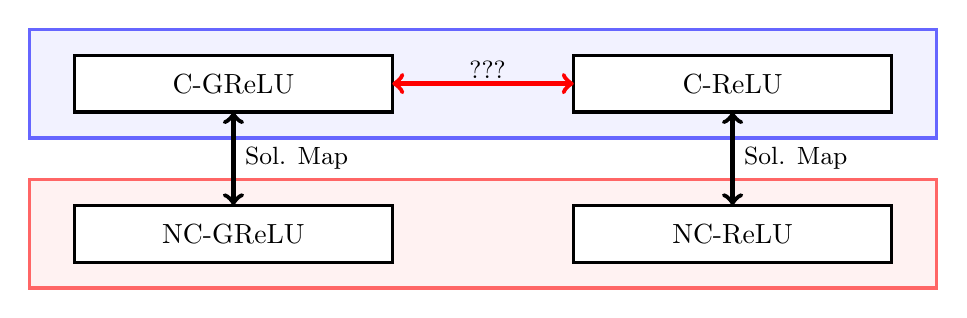
\begin{tikzpicture}[scale=1,
	]
	\begin{axis}[width=1.1\linewidth, height=5cm,
			axis lines=none,  % don't print axis lines
			yticklabels={,,}, xticklabels={,,},
			ymin=-0.2, ymax=10.2, x axis line style={-},
			xmin=-0.2, xmax=20.2, y axis line style={-},
		]

		\filldraw[color=blue!60, fill=blue!5, line width=0.4mm](axis cs:0,5.8) rectangle (axis cs:20, 10);
		\filldraw[color=red!60, fill=red!5, line width=0.4mm](axis cs:0,0) rectangle (axis cs:20, 4.2);

		% non-convex models
		\filldraw[line width=0.4mm, fill=white](axis cs:1,1) rectangle (axis cs:8, 3.2) node[pos=.5] {NC-GReLU};
		\filldraw[line width=0.4mm, fill=white](axis cs:12,1) rectangle (axis cs:19, 3.2) node[pos=.5] {NC-ReLU};

		% convex models
		\filldraw[line width=0.4mm, fill=white](axis cs:1,6.8) rectangle (axis cs:8, 9) node[pos=.5] {C-GReLU};
		\filldraw[line width=0.4mm, fill=white](axis cs:12,6.8) rectangle (axis cs:19, 9) node[pos=.5] {C-ReLU};

		\draw [<->, solid, draw=black, line width = 0.6mm] (axis cs:4.5,3.2) -- (axis cs:4.5,6.8) node[right, pos=0.5] {\small Sol. Map};

		\draw [<->, solid, draw=black, line width = 0.6mm] (axis cs:15.5,3.2) -- (axis cs:15.5,6.8)  node[right, pos=0.5] {\small Sol. Map};

		%\draw [<-, solid, draw=black, line width = 0.6mm] (axis cs:6,9) to [bend left=15] (axis cs:14, 9);

		\draw [<->, solid, draw=red, line width = 0.6mm] (axis cs:8,7.9) -- (axis cs:12,7.9);
		\node[align=center] at (axis cs:10.1, 7.8) {\small \red{???} \\};
	\end{axis}

\end{tikzpicture}%
